%\documentclass{article}
%\usepackage{graphicx,subfigure}
%\usepackage{caption,rotating}
%\begin{document}

\begin{figure}[p]
\centering
 \subfigure[Plate (i) Sheep w479 Wrinkled]{
    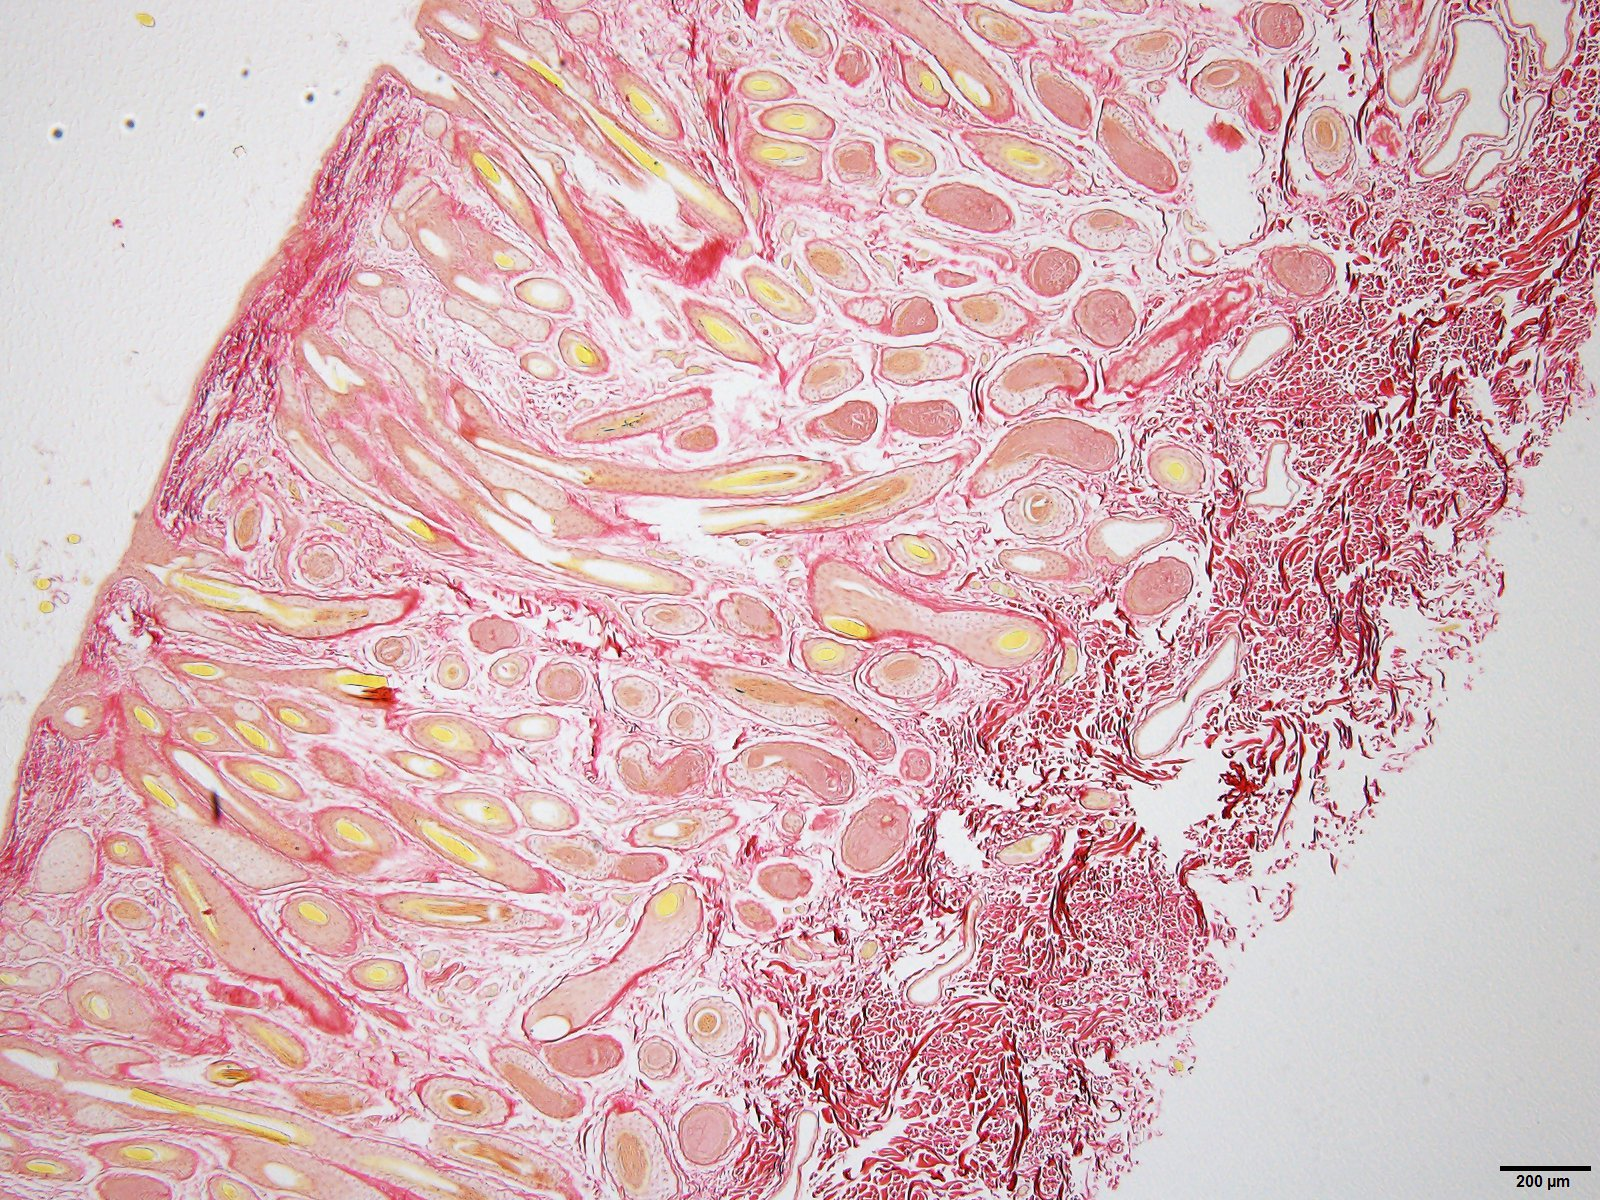
\includegraphics[scale=0.20]{w479-2-rigid.jpg}
  }
 \subfigure[Plate (ii) Sheep w490 Wrinkle-free]{
    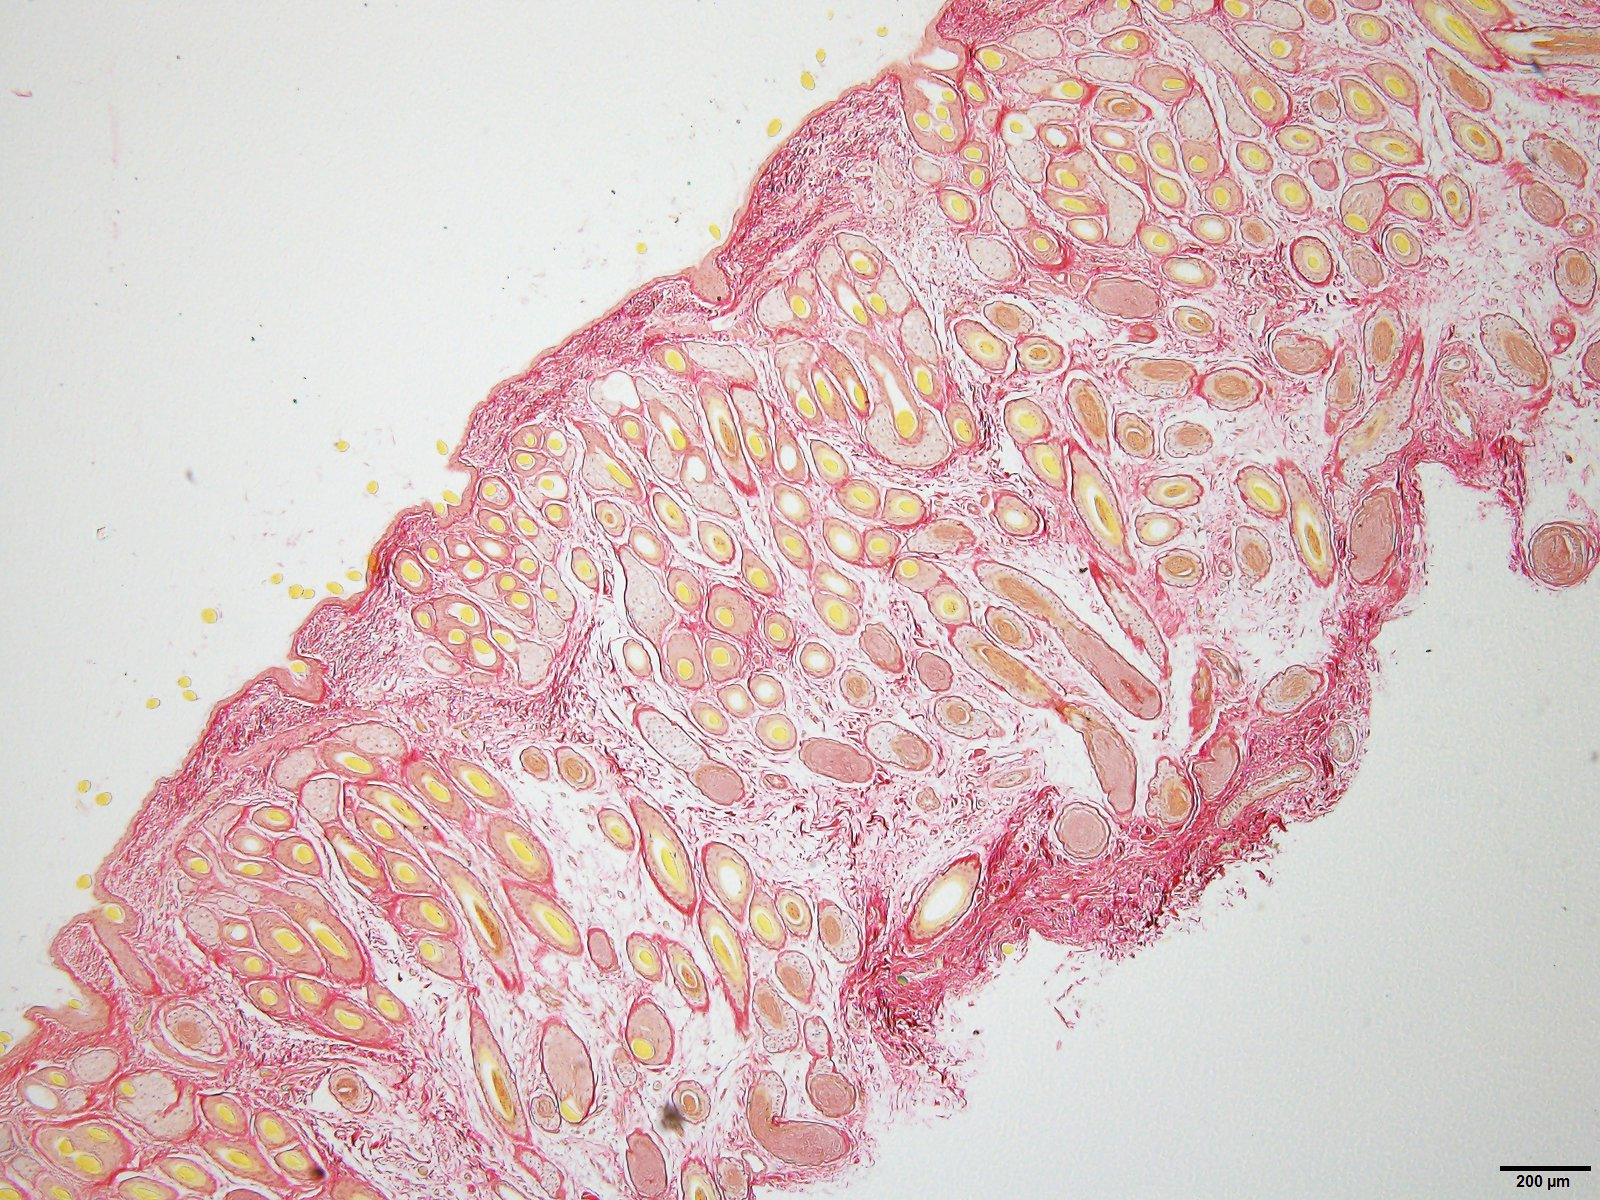
\includegraphics[scale=0.20]{w490-2-supple.jpg}
  }
  \caption{Vertical sections from a wrinkled (i) and a wrinkle-free (ii)  sheep from Trial 1 flock 2 stained with PSR and examined with a 4x objective. These are the same two sections as shown with polarised light in Figure~\ref{fig:polar}. }
\vfill
  \label{fig:nopolar}
\end{figure}

%\end{document}

